
\subsection{Answers}
\begin{table}[htb]%
\begin{center}%
\caption{Q12: Which MPI implementations do you use?}%
\label{tab:Q12-ans}%
\begin{tabular}{l|l|r}%
\hline%
Choice & Abbrv. & \# Answers \\%
\hline%
Open MPI & OMPI & 723 (85.4\%) \\%
Intel MPI & Intel & 522 (61.6\%) \\%
MPICH & MPICH & 470 (55.5\%) \\%
MVAPICH & MVA & 175 (20.7\%) \\%
Cray MPI & Cray & 145 (17.1\%) \\%
IBM MPI (BG/Q, PE, Spectrum) & IBM & 92 (10.9\%) \\%
Fujistu MPI & Fujitsu & 29 (3.4\%) \\%
MS MPI & MS & 27 (3.2\%) \\%
HPE MPI & HPE & 23 (2.7\%) \\%
NEC MPI & NEC & 23 (2.7\%) \\%
I do not know & No idea & 10 (1.2\%) \\%
MPC MPI & MPC & 8 (0.9\%) \\%
Sunway MPI & Sunway & 5 (0.6\%) \\%
Tianhe MPI & Tianhe & 3 (0.4\%) \\%
other & - & 27 (3.2\%) \\%
\hline%
\multicolumn{2}{c}{total} & 2282 (847)\\%
\hline%
\end{tabular}%
\end{center}%
\end{table}%


\subsection{List of other answers}

Looking more precisely at the 27 other MPI implementations
specifically mentioned in the answers, points to lesser known MPI
implementations with an existing, but usually geographically
constraint, user base. Such examples are Bull~MPI and MadMPI (both
with 4 mentions in Europe:France) and ParaStation~MPI (10 mentions in
Europe:Germany). Out of them only one MPI implementation stands out
with a more international user base, SGI MPI with 5 total
mentions. Finally, for the sake of completeness it should be noted
that some MPI implementations were mentioned at least once (Sun~MPI,
Adaptive~MPI, PGI~MPI, Platform~MPI) as well as a Python API for MPI
(mpi4py). 

\mycomment[AH]{I do not think they are geographically constrained, but
vendors force users to use their MPI. For example, BG/* users have no
choice but using IBM MPI, the K users must use Fujistu MPI.}.

\mycomment[AH]{It would be nice to categorize MPI implementations into
two; proprietary (vendor) MPI and public domain MPI}.

\begin{report}
\begin{itemize}
\item Europe:France: BULL MPI
\item Europe:France: BULLMPI
\item Europe:France: BullMPI
\item Europe:France: BullX-MPI
\item Europe:France: MadMPI
\item Europe:France: MadMPI
\item Europe:France: Platform
\item Europe:France: SGI MPI
\item Europe:France: madMPI
\item Europe:France: madmpi
\item Europe:France: mpi4py
\item Europe:Germany: ParaStation MPI
\item Europe:Germany: ParaStation MPI
\item Europe:Germany: ParaStation MPI
\item Europe:Germany: ParaStation MPI
\item Europe:Germany: ParaStation MPI
\item Europe:Germany: ParaStation MPI
\item Europe:Germany: ParaStation MPI
\item Europe:Germany: ParaStation MPI
\item Europe:Germany: ParaStation MPI
\item Europe:Germany: ParaStation MPI
\item Europe:Germany: Sun MPI
\item Europe:UK: SGI MPT
\item Japan: SGI MPI
\item Russia: SGI MPI
\item USA: Adaptive MPI
\item USA: PGI MPI

\end{itemize}
\end{report}

\begin{figure}[htb]
\begin{center}
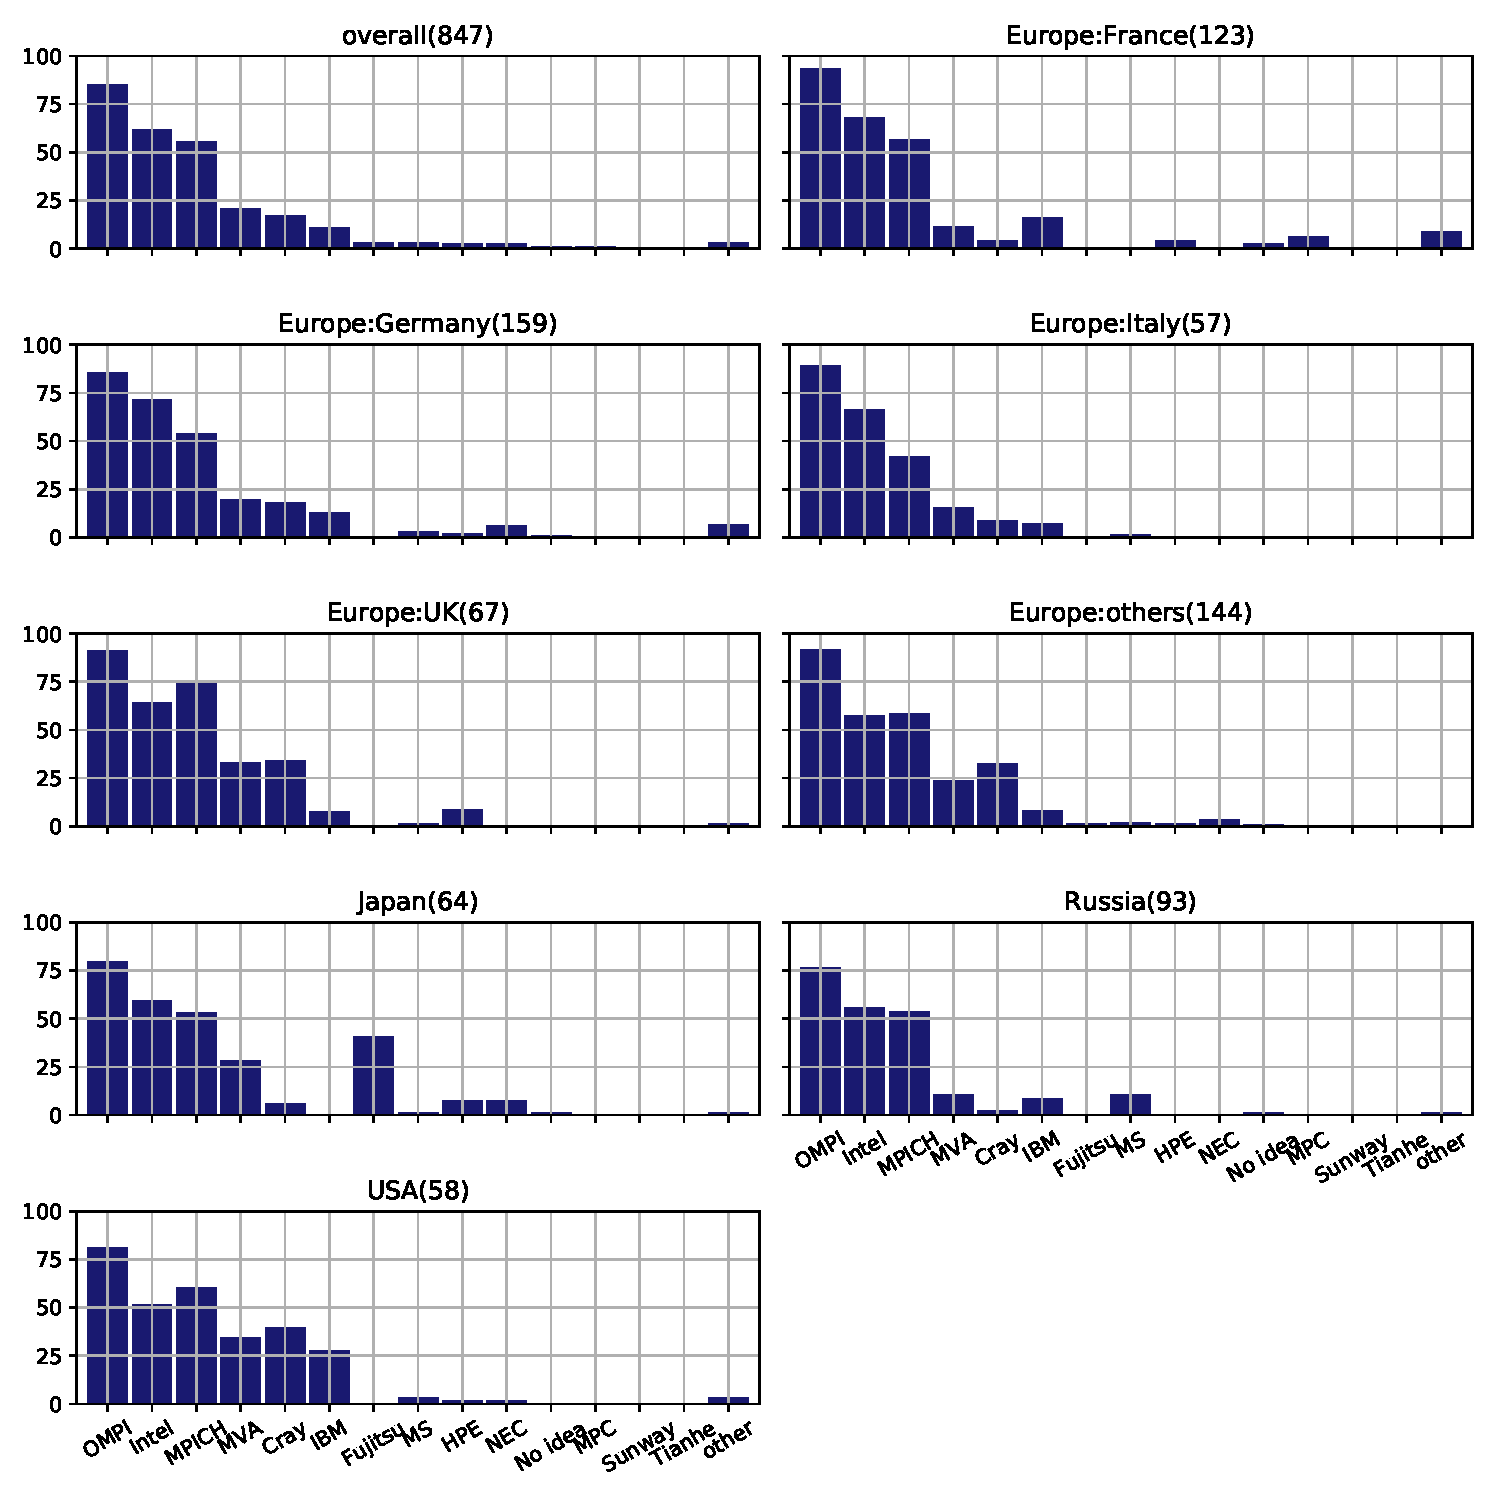
\includegraphics[width=10cm]{../pdfs/Q12.pdf}
\caption{Breakdown of MPI implementation usages per location}
\label{fig:Q12}
\end{center}
\end{figure}

\subsection{Comments}

Open MPI, Intel MPI and MPICH dominates more than 60 \%.
